%----------------------------------------------------------
% PACKAGES AND THEMES
%----------------------------------------------------------
\documentclass[aspectratio=169,xcolor=dvipsnames,handout]{beamer}

\usetheme{Darmstadt}
\usecolortheme{seahorse}
\setbeamercovered{transparent}

\usepackage[hangul]{kotex}
\usepackage{hyperref}
\usepackage{graphicx, array, adjustbox, makecell}
\usepackage{booktabs, multicol, multirow}

% font조정
%\usepackage{fontspec}
%\setmainfont{Times New Roman}
%\setmainhangulfont{NanumGothic}

% 문자열 대체{노사관계론 전용}
\usepackage{newunicodechar}
\newunicodechar{•}{$\cdot$}
\newunicodechar{➔}{$\implies$}
\newunicodechar{∴}{$\therefore$}
\newunicodechar{∵}{$\because$}

%----------------------------------------------------------
% TITLE PAGE
%----------------------------------------------------------
\title{노사관련 국제기구}
\subtitle{노사관계의 이론과 실제}
\author{오성재}
\institute[CNU]
{\relax
    충남대학교 경제학과\
    }
\date{2024년 11월 18일}

%----------------------------------------------------------
\begin{document}
%----------------------------------------------------------

\frame{\titlepage}

\begin{frame}{목차}
    \small
    \tableofcontents[hideallsubsections]
\end{frame}

\section{주요국의 고용관계}%
\begin{frame}[allowframebreaks]
    \frametitle{국가별 고용관계}
    \begin{itemize}[<+->]
        \item 노사자율주의 Voluntarism: 영국, 미국
        \begin{itemize}
            \item 대립적 단체교섭형
\begin{itemize}
               \item 정부는 민간기업 고용관계에 가급적 불개입
               \item 노사대등한 입장에서 교섭과 조정
               \item 노사대등한 단체협약 체결
\end{itemize}
        \end{itemize}
        \item 정치적 조합주의 Political Unionism: 프랑스, 이탈리아
        \begin{itemize}
            \item 강한 이데올로기의 영향
\begin{itemize}
               \item 노조는 사용자와 감정을 달리하는 이질적 집단 취급
               \item 노조 생성시부터의 계급투쟁적 색채 농후
               \item 사용자는 권위적 가부장적 경영스타일
               \item 전국적 또는 개별기업에서도 계급투쟁적 활동의 전개
\end{itemize}
        \end{itemize}
        \item 민주적 조합주의 Democratic or Societal Corporatism: 독일, 스웨덴
        \begin{itemize}
            \item 공동체 의사결정형, 경영참가형
\begin{itemize}
               \item 노사가 근로조건을 공동결정
               \item 노사쌍방의 신의 성실의무 이행약속
               \item 산업민주화 방향, 경영참가제 실시, 성과배분제의 제도화
\end{itemize}
        \end{itemize}
        \item 기업조합주의 Micro corporatism: 일본
        \begin{itemize}
        \item 가족주의의 공동체원리, 집단주의의 화합원리
            \item 유교적 집단주의 공동체형성 노사관계 $\implies$ 화합적 의사결정
\begin{itemize}
               \item 기업별 노조시스템
               \item 종신고용제 $\implies$ 근로자의 직업안정
               \item 연공서열 임금제
\end{itemize}
        \end{itemize}
        \item 국가조합주의 State Corporatism: 남미, 개도국 등
        \begin{itemize}
            \item 강력한 국가개입주의
\begin{itemize}
               \item 4정부의 주도적 역할 강조 노동기본권 제한
               \item 협력적 고용관계 구축을 위한 입법 제정
\end{itemize}
        \end{itemize}
        \item 공산권 Stalinist Unionism:
        \begin{itemize}
            \item 공산당의 정책 우선, 경제성장우선주의
\begin{itemize}
               \item 노조는 근로자 대변기구라기 보다는 생산독려자 역할 수행
               \item 노조가 당의 한 기구이며 노조 설립 강제
\end{itemize}
        \end{itemize}
    \end{itemize}
\end{frame}

\begin{frame}[allowframebreaks]
    \frametitle{영국의 고용관계}
    \begin{itemize}[<+->]
        \item 노동조합의 특징
        \begin{itemize}
            \item 한 기업 (또는 산업) 내에 다수의 조합 혼재: 복수노동조합 (multi-unionism)
            \item 취업 전 또는 직후에 노동조합에 가입해야 하는 closed shop 인정
            \item 유일한 전국중앙조직인 ‘영국노동조합회의 (Trade Union Congress: TUC)’ 존재
        \end{itemize}
        \item 1906년 거래분규법 (Trade Dispute Act) 제정 
        \begin{itemize}
            \item 형법, 민법의 여러 분야에서 노조에 대한 면책특권 부여  
        \end{itemize}
    \framebreak%
        \item 영국의 노사자율주의의 특징
        \begin{itemize}
            \item 단체협약은 법적으로 양 당사자에 강제적이지 않음
            \item 사용자의 노조 인정은 자발적 (∴노조를 인정하는 행정적•사법적•일반적 절차 없음) 
            \item 국가에서 제공하는 분쟁조정절차: 보조적, 강도가 약함, 자발적 성격
            \item 정부는 파업을 중지시키거나 냉각기간을 설정할 권한을 가지고 있지 않음
        \end{itemize}
        \item 1979년 대처수상은 신자유주의 도입하여 노조의 기득권과 세력을 축소
        \item 2000년이후에도 시장주의를 노사관계에 도입하는 정책의 큰 틀이 지속되면서 노조의 위축현상이 계속됨
    \end{itemize}
\end{frame}

\begin{frame}[allowframebreaks]
    \frametitle{미국의 고용관계}
    \begin{itemize}[<+->]
        \item 환경
        \begin{itemize}
            \item 공화당과 민주당의 안정적인 양당 체제 유지
            \item 경제상황: 상승과 하락의 사이클 반복 경향
            \item 고용관계 특징: 주별로 비교적 독립적인 산업정책 추진 $\implies$ 분권화 경향
            \begin{itemize}
                \item 미시건 주: 자동차산업이 왕성하여 노조원도 많고 노조의 영향력도 큼
                \item 미시시피, 알라바마 등 남부의 소득이 낮은 주 (Deep South): 조합원도 적고 노조의 힘도 약함
            \end{itemize}
            \item 고용형태:
            \begin{itemize}
                \item 노조 조직부문 (unionized sector): 노사간 대립관계, 
                \item 노조 미조직부문 (non-union sector): 사용자의 광범위한 재량권과 통제권 인정
            \end{itemize}
        \end{itemize}
    \framebreak%
        \item 미국의 노동조합
        \begin{itemize}
            \item 노동조합 연맹, 직종별•산별 노조 및 노동조합지부 등 삼층구조로 구성 
            \item 단체협약: 대부분 사업장별•지역별 노동조합지부에서 실시
            \item 특징
            \begin{itemize}
                \item 주로 실리적 경제적 노동운동 (노동조합의 목적), 잘 발달된 단체교섭제도 $\implies$ 대립적 노사관계
                \item 직무통제 조합주의를 통한 노조의 영향력 강함
                \item 임금과 근로조건 향상을 중시하고 정치와 경영에 관심을 두지 않는 노조 (Bread and Butter Unionism)
            \end{itemize}
        \end{itemize}
    \framebreak%
        \item 사용자 단체: 전국제조업협회 (American National Association of Manufacturing) 또는 상공회의소 (Chamber of Commerce)의 전국본부 혹은 지부 등이 사용자의 대변역할 수행
        \item 정부의 주요 역할
        \begin{itemize}
            \item 개별적인 노사관계의 차원에서 고용조건에 대한 직접적 규칙제정의 역할: 고용차별, 산업안전보건, 실업보험, 최저임금, 최장노동시간 및 퇴직부문 등에 대한 규칙 제정 $\implies$ 민간부문의 단체협상에 직접 개입하지 않음
            \item 공공부문 사용자로서의 역할
        \end{itemize}
    \end{itemize}
\end{frame}

\begin{frame}[allowframebreaks]
    \frametitle{일본의 고용관계}
    \begin{itemize}[<+->]
        \item 환경
        \begin{itemize}
            \item 정치제도: 입헌군주제이며 자유민주당 (자민당)이 장기간 집권
            \item 경제환경:  
            \begin{itemize}
               \item 1950--1980년대까지 고도성장
               \item 1990년대 초반부터 2000년대까지 경제침체, 2010년이후 경제성장률이 1\%대로 회복되는 추세
               \item 장기 침체 과정에서 20년 이상 임금인상 정체되어 임금수준은 국민소득에 비하면 낮은 수준
            \end{itemize}
            \item 사회적•경제적 환경 급변: 인구의 고령화, 고학력 근로자의 증가, 여성의 노동시장 참여 증대, 외국인 근로자의 이주 증대
            \begin{itemize}
               \item 2020년 `동일노동 동일임금 규칙'을 법제화
               \item 2021년에 `정년 70세 권고안' 국회 통과
            \end{itemize}
        \end{itemize}
    \framebreak%
        \item 노동조합
        \begin{itemize}
            \item 조직형태로 볼 때 기업별 조직이 많으며 산별 및 직업별 조합은 소수
            \begin{itemize}
                \item 기업별 노조는 상호 협상력을 보완하기 위해 슌토 (春鬪)의 관행을 유지 
            \end{itemize}
            \item 전국적 중앙조직
            \begin{itemize}
                \item 렌고 (連合): 1989년 출범, 2020년 현재, 1천만 여명의 조합원 가입, 공공부문 및 민간부문 포함 미국의 AFL-CIO, 영국의 TUC에 이어 세계 3위의 노조
                \item 젠로렌 (全勞聯): 1989년 결성, 약 51만 명 조합원 
                \item 젠로코 (全勞協): 9만 명의 조합원
            \end{itemize}
            \item 일본 노동조합의 특징: 기업과 밀착되어 있으며 기업 정책에 협조적
        \end{itemize}
    \framebreak%
        \item 사용자단체
        \begin{itemize}
            \item 케이단렌 (日本經濟團體連合會): 직접 협상에 참여하지 않고 정부에 대한 로비, 산하기업에 대한 교육과 자문 등의 역할
            \item 일본 사용자의 특징 
            \begin{itemize}
                \item 가부장적 온정주의적 성향이 강하고 집단의 이익을 우선시 함
                \item 대기업의 경우 전통적으로 정규직 직원에 대한 장기고용과 연공서열임금제 유지. (단, 중소기업이나 비정규직 직원에게는 그렇지 않음) 
            \end{itemize}
            \item 연공급의 단점 (예: 인건비가 매년 커지는 경직성을 갖고 준고정비용화)의 해소방안
            \begin{itemize}
                \item 1970년대 오일쇼크 후 직능급 (직무수행능력에 따라 직능등급을 설정하여 차등 급여 지급) 도입
                \item 1990년대이후 연공급이 위축되고 성과급이 확산되는 추세가 2020년대에도 지속됨 
            \end{itemize}
        \end{itemize}
    \framebreak%
        \item 정부: 후생노동성이 담당. 분권적 고용관계 유지 및 기업중심의 형태를 유지하도록 유도.
        \begin{itemize}
            \item 2차 세계대전 이후 미국식 고용관계 모델 도입 후 일본 정부도 정책기조 유지
            \begin{itemize}
                \item 일본 정부는 고용관계를 분권적이며 기업중심의 형태로 유지하고자 하는 반면, 고용문제에 대한 주요 의사결정은 노•사•정 3자로 구성된 각종 위원회 결정: 협조적인 전통 유지
            \end{itemize}
            \item 기업조합주의 (Micro-Corporatism): 정부가 개별기업의 고용관계에 거의 개입하지 않는 반면, 기업내부에서는 노사가 합의와 협조에 의한 의사결정 
        \end{itemize}
    \end{itemize}
\end{frame}

\begin{frame}[allowframebreaks]
    \frametitle{싱가포르의 고용관계}
    \begin{itemize}[<+->]
        \item 환경
        \begin{itemize}
            \item 정치체제: 인민행동당이 거의 유일한 정당
            \item 경제적 환경: 자원과 자본이 부족한 도시국가로 전자산업과 외국기업에 대한 의존도가 높음
                \begin{itemize}
                    \item 세계 경기의 움직임에 따라  큰 폭의 부침을 거듭
                    \item 전통적으로 실업률 낮음
                \end{itemize}
            \item 고용관계 환경  (Bread YES\@; Voice NO)
                \begin{itemize}
                    \item 고용안정, 능력개발, 복지제공 등 정부가 노동자복지를 직접 제공 (긍정적 측면)
                    \item 노동3권의 제한과 국가의 임금억제 (부정적 측면) 
                \end{itemize}
        \end{itemize}
    \framebreak%
        \item 노동조합
        \begin{itemize}
            \item 복수노조는 사실상 불허
            \item 전국단위의 유일한 노조는 전국노동조합회의 (NTUC)
            \begin{itemize}
                \item NTUC 출신 간부가 인민행동당의 주요 당직을 맡을 정도로 정당과 노조가 긴밀한 관계 유지
                \item 싱가포르노동재단 (SLF)이라는 공익재단을 설립하여 산업재해자 구호, 장학금 지급, 휴양시설 제공 등의 서비스 제공  
            \end{itemize}
            \item 1987년 이후 30여년간 파업이 거의 발생하지 않음
            \begin{itemize}
                \item 강력한 국가개입주의, 파업에 대한 법률적 제한 (예: 조합원 2/3 이상의 비밀투표에 찬성해야 파업 가능), 노조의 생산주의적 협력주의적 특성
            \end{itemize}
        \end{itemize}
    \framebreak%
        \item 사용자단체: 싱가포르전국사용자연맹 (SNEF) 
        \begin{itemize}
            \item 유일 사용자단체로 NTUC의 주된 상대역
            \begin{itemize}
                \item 단체교섭에 참여하지 않으며 가맹회원에 대한 자문, 훈련 및 개발, 정보제공 등의 서비스 제공, 노동법 자문, 노사관계 지침, 단체교섭에 대한 권고, 사용자의견 대변 등의 역할 수행
            \end{itemize}
            \item 그 외에도 싱가포르해운사용자연맹, 싱가포르인쇄미디어협회 등이 있음
        \end{itemize}
        \item 정부
        \begin{itemize}
            \item 고용관계의 기본 규칙이나 법적제고 형성 및 분쟁해결을 위한 서비스제도 감독
            \item 민간의 단체교섭에도 깊이 개입하고 단체협약의 합의가 실패할 경우 산업중재재판소에서 중재하고 그 결정은 최종적인 집행력을 갖춤
            \item 정부는 임금조정을 수행하는 NWC에서 주도적인 역할을 수행하여 임금수준을 규율
        \end{itemize}
    \end{itemize}
\end{frame}

\begin{frame}[allowframebreaks]
    \frametitle{중국의 고용관계}
    \begin{itemize}[<+->]
        \item 환경
        \begin{itemize}
            \item 정치체제: 공산당 일당독재 국가
            \item 경제적 환경: 인구 13억 8천만여 명, 국토면적은 세계 3위 (한반도의 44배)
            \begin{itemize}
                \item 2000년부터 2010년까지 연평균 경제성장률이 10.3\%, 2011년부터 하락하기 시작하여 2016--19년에 6\%대를 보이다가 2020년에 코로나19 영향으로 2.2\%로 하락
                \item 2008년에 신노동법 (노동계약법)이 발효되면서 고용안정 강화와 임금상승 추진
                \item 비교적 양질의 노동력 보유 
            \end{itemize}
            \item 고용관계 환경: 최근 노동쟁의 급증
            \begin{itemize}
                \item 노동쟁의 양상도 파업. 집단행진, 피켓팅 등에서 점거농성, 폭력시위 등으로 극렬화
            \end{itemize}
        \end{itemize}
    \framebreak%
        \item 공회 (노동조합)
        \begin{itemize}
            \item 공회: 일정규모 이상의 모든 기업에서 공회를 설립하도록 강제 $\implies$ 자율권이 거의 없고 공산당의 지시와 통제를 받는 전통적인 레닌스타일의 노동조합주의
            \begin{itemize}
                    \item 대립적 노사관계를 추구하지 않으며 노사협의회 정도의 기능을 수행
            \end{itemize}
            \item 설립된 공회는 중앙조직인 중국총공회 (All-China Federation of Trade Unions: ACFTU)에 가입해야 함
            \begin{itemize}
                    \item 중국총공회는 당의 지시를 노조원들에게 전달하는 전달벨트 (transmission belt)의 역할을 주로 수행. 즉 근로자 대변기능보다는 당의 선전기구 또는 생산독려자의 역할
            \end{itemize}
            \item 단체교섭: 기업별, 지역별 및 업종별로 가능하나 기업별 교섭이 가장 많음
            \begin{itemize}
                    \item 정부가 정해준 임금인상률에 의존하는 결정
            \end{itemize}
        \end{itemize}
    \framebreak%
        \item 사용자 단체
        \begin{itemize}
            \item 공식적 사용자단체는 없으며 사용자는 대체로 수동적 태도 견지
        \end{itemize}
        \item 정부
        \begin{itemize}
            \item 전통적인 공산주의 국가의 특징이 남아 있어서 공산당과 정부가 고용관계에 절대적인 영향력을 행사 
            \item 중국총공회를 통하여 당의 지시를 근로자에게 전달
            \item 중국 노동자들의 단체행동은 공회 (노조) 개입으로 해소되는 사례는 극소수이며, 절반 이상은 단체교섭, 37\%는 정부가 개입하여 조정 및 중재로 마무리
        \end{itemize}
    \end{itemize}
\end{frame}


\section{국제노사정기구}
\subsection{국제노사조직}
\begin{frame}
    \frametitle{국제노동자조직}
    \begin{itemize}[<+->]
        \item 자본의 세계하에 대응하여 국경을 초월한 노동조합의 연대활동을 강조하기 위해 설립
        \item 국제노동조합조직으로는 정치적 이념에 따라 차이를 나타내는데 현재에는 
        \begin{itemize}
            \item 국제자유노련 (International Trade Union Confederation: ITUC): 미국 영국중심, 시장경제 지향, 주도적 역할
            \item 세계노동조합연맹 (World Federation of Trade Union: WFTU): 공산권국가중심, 소련붕괴후 위축
            \item 경제협력개발기구 (OECD) 내 노조의 견해를 반영하도록 하는 노동조합자문회의 (Trade Union Advisory Committee to the OECD) 등이 있음
        \end{itemize}
    \end{itemize}
\end{frame}

\begin{frame}
    \frametitle{국제사용자조직}
    \begin{itemize}[<+->]
        \item 노동조합의 성장에 대항하기보다는 국제적 정부기관의 발전에 대한 대응으로 창설
        \item 국제노동조합조직보다 역사가 일천하고 역할이 상대적으로 미미
        \item 대표적 기구는 아래와 같음
        \begin{itemize}
            \item 국제사용자기구 (International Organisation of Employers: IOE)
            \item 비즈니스유럽 (Business Europe)
            \item 유럽산업연맹 (Union des Industries del la Communaute Europeenne: UNICE)
            \item OECD 내 기업•산업자문위원회 (Business and Industry Advisory Committee to the OECD)등
        \end{itemize}
    \end{itemize}
\end{frame}

\subsection{국제노동기구}%

\begin{frame}[allowframebreaks]
    \frametitle{국제노동기구}
    \begin{itemize}[<+->]
        \item 국제노동기구 (International Labor Organization: ILO)는 정부•사용자•노동조합의 고용관계에 대한 국제적 활동을 위한 기구
        \item 1919년 베르사이유 평화조약에 의해 설립
        \item 현재 국제연합 (UN)의 노동문제에 대한 전문기관으로 187개의 회원국으로 구성
        \item 주요 기능
        \begin{itemize}
            \item 국제적 근로기준의 발전에 기여: 국제노동법 및 국제비교고용관계 자료의 주요 원천 181개 이상의 협약과 188개의 권고를 채택하고 6,433개 이상의 비준을 받음       
            \item 국제적 인사정책 및 관행에 대한 중요 정보원천: 특정기준의 준수를 강요 않으며 정부에 위임
        \end{itemize}
        \item 우리나라는 1991년 12월 9일 ILO사무총장에게 ILO헌장 수락서 제출$\implies$152번째 회원국 
        \item 한국은 ILO 가입 30년 만인 2021년 4월에 정부가 제출한 ILO 핵심협약 제87호, 98호, 29호를 국회 비준   
    \end{itemize}
\end{frame}

\begin{frame}[allowframebreaks]
    \frametitle{ILO 규약 및 비준 협약}
    \begin{itemize}[<+->]
        \item 비준 장려 협약 (37)
        \begin{itemize}[<+->]
            \item 핵심협약 (8) (core conventions)
            \begin{itemize}
                \item 결사의 자유관련: 87호 (결사의 자유 및 단결권보호), 98호 (단결권 및 단체교섭권보호)
                \item 강제근로관련: 29호 (강제노동금지), 105호 (강제노동폐지)
                \item 차별금지관련: 100호 (균등대우), 11호 (고용 및 작업장 차별금지)
                \item 아동근로: 138호 (근로가능최저연령), 182호 (가혹행위금지)
            \end{itemize}
        \end{itemize}
        \begin{itemize}[<+->]
            \item 우선협약 (4) (priority conventions)
            \begin{itemize}
                \item 근로감독관련: 81호 (근로감독), 129호 (근로감독 (농업))
                \item 고용정책: 122호
                \item 3자협의: 144호
            \end{itemize}
        \end{itemize}
    \framebreak%
        \begin{itemize}[<+->]
            \item 기타 비준장려 협약 (25)
            \begin{itemize}
                \item 주휴관련: 공장 (14호), 상업 및 사무소 (106호)
                \item 산업안전보건: 농원근로자 (110호), 방사선 (115호), 기계방호 (119호), 사무실위생 (120호), 직업성암 (139호), 작업환경 (148호), 부두작업 (152호), 산업안전보건 (155호) 
                \item 사회보장: 고령 및 유족보상 (128호), 의료보호 (130호), 사회보장 (157호)
                \item 최저임금: 최저임금결정 (131호)
                \item 유급휴가: 유급휴일 (132호), 유급교육휴가 (140호)
                \item 근로자대표: 135호
                \item 인적자원개발: 142호 ('94.1, 비준)
                \item 노동행정: 150호 (97. 12. 비준)
                \item 공공부문 노사관계: 151호
                \item 휴식: 도로운송 근로시간 및 휴식시간 (153호)
                \item 단체교섭: 154호
                \item 가족부양: 가족부양 근로자 (156호)
                \item 해고: 고용종료 (158호)
                \item 직업재활: 장애인직업재활 및 고용 (159호)
            \end{itemize}
        \end{itemize}
        \begin{itemize}
            \item 일반비준대상 협약 (176): 노동통계 (160호), 선원의 건강진단에 관한 협약 (13)외 174개
        \end{itemize}
    \end{itemize}
\end{frame}

\begin{frame}[allowframebreaks]
    \frametitle{협약 비준현황}
    \centering
    \begin{figure}[ht]
        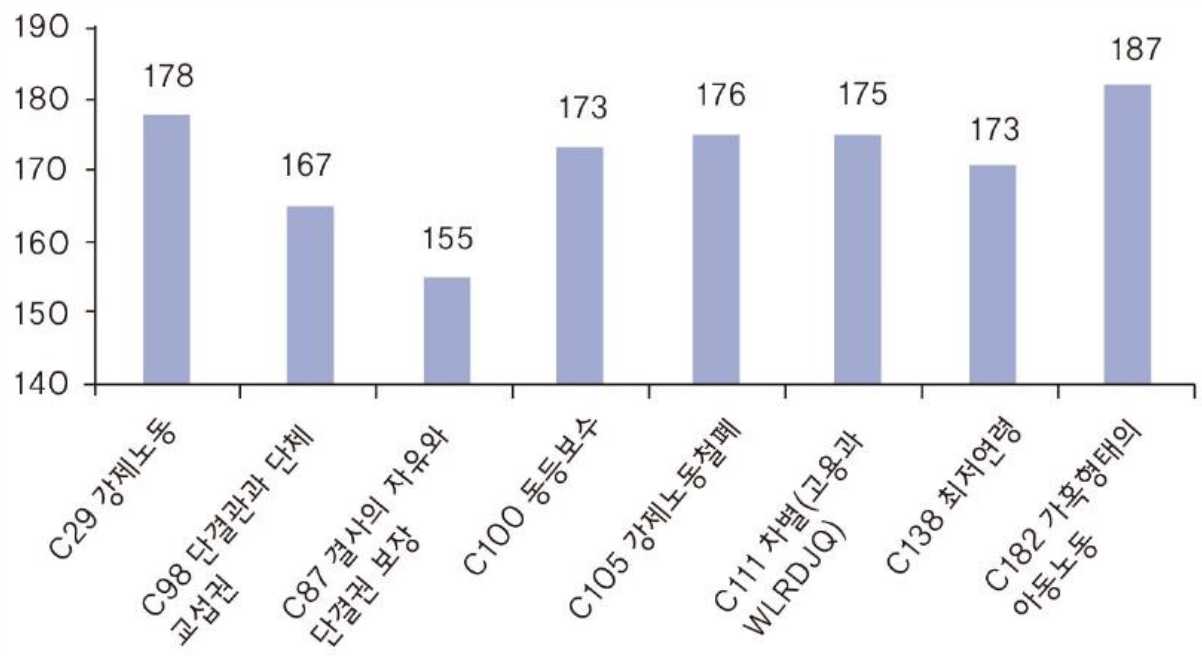
\includegraphics[width=.6\textwidth]{pic/ILO핵심협약}
        \caption{핵심협약 비준현황}
    \end{figure}
    \centering
    \begin{figure}[ht]
        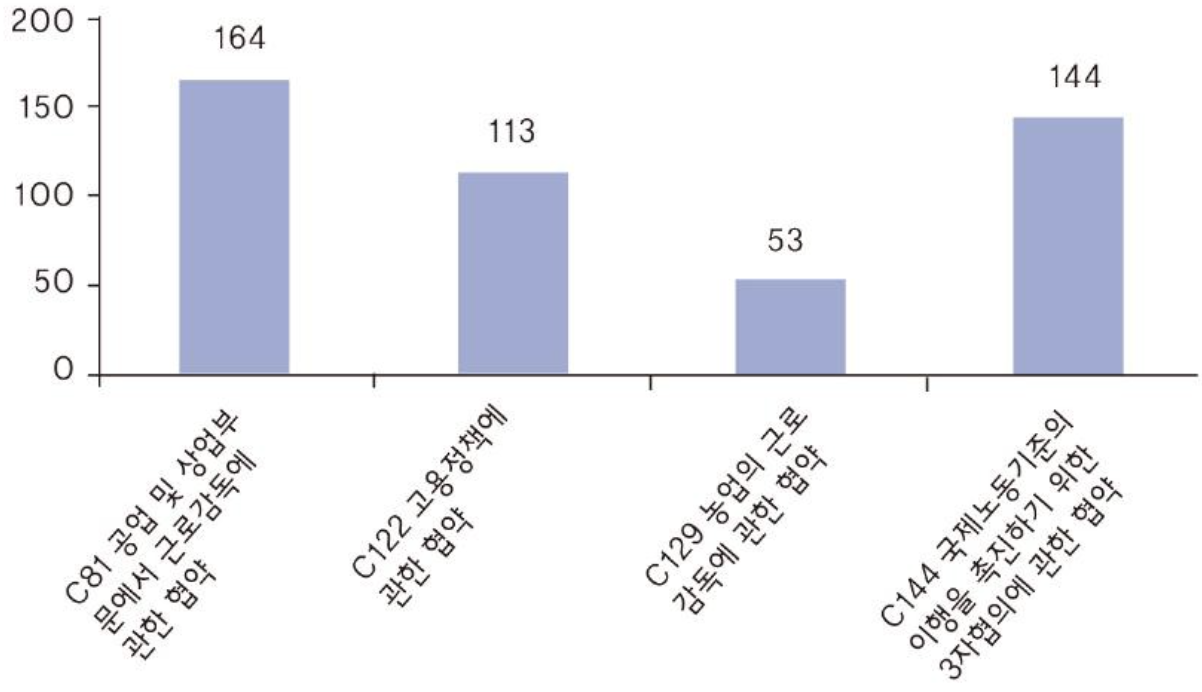
\includegraphics[width=.6\textwidth]{pic/ILO우선협약}
        \caption{우선협약 비준현황}
    \end{figure}
\end{frame}

\subsection{우리나라의 비준 협약 내용}%
\begin{frame}
    \frametitle{우리나라 비준 협약 내용}
    \begin{itemize}[<+->]
        \item 2022년 11월 현재 32개 협약 비준
        \begin{itemize}
            \item 핵심협약:  제138호 (취업상 최저연령), 제182호 (가혹 아동노동 철폐), 제100호 (남녀동일노동·동일임금), 제111호 (고용 및 직업상 차별금지)에 이어서 2021년에 국회가 29호 (강제 노동 금지), 87호 (결사의 자유), 98호 (단결권 및 단체교섭권 장려)  비준하여 7개 협약
            \item 105호 (강제노동폐지)는 비준하지 않음
            \item 우선협약: 제81호 (근로감독), 제122호 (고용정책), 제144호 (3자협의) 등 3개 협약
            \item 기타 비준장려협약: 제106호 (사업과 사무) 등
            \item 일반기준대상협약: 제2호 (실업) 등
        \end{itemize}
    \end{itemize}
\end{frame}

\begin{frame}
    \frametitle{우리나라 비준 협약 내용 국제 비교}
    \begin{itemize}[<+->]
    \item 한국의 협약 비준 수준은 미국 (14개)보다 높지만 영국 (87개), 프랑스 (124개), 독일 (85개) 및 일본 (49개) 등과 비교하여 낮은 수준
    \end{itemize}
    \begin{table}
        \centering
        \resizebox{.6\textwidth}{!}{\relax
            \begin{tabular}{@{}lcccccc@{}}
\toprule
 & \textbf{영국} & \textbf{미국} & \textbf{프랑스} & \textbf{독일} & \textbf{일본} & \textbf{한국} \\ 
\midrule
핵심협약(총 8개) & 8 & 2 & 8 & 8 & 6 & 7 \\
우선협약(총 4개) & 3 & 1 & 4 & 4 & 3 & 3 \\
그 외(총 177개)  & 76 & 11 & 112 & 73 & 40 & 22 \\
\midrule
\textbf{계}       & 87 & 14 & 124 & 85 & 49 & 33 \\
\bottomrule
\end{tabular}

        }
        \caption{주요국의 ILO 협약 비준 현황}
    \end{table}
\end{frame}

\begin{frame}
    \frametitle{핵심협약 87호}
    \begin{itemize}[<+->]
        \item 87호 결사의 자유 협약 비준을 위한 노조법, 공무원노조법, 교원노조법 등 3개 법률의 개정안은 2019년 10월 1일 국무회의에서 다음과 같이 심의 의결
        \begin{itemize}
                \item 노조법 개정안: 실업자·해고자도 기업별 노동조합 가입 허용. 노조 임원자격은 노동조합 규약으로 자율적으로 결정. 노조 전임자 급여 지급금지 규정 삭제 등
                \item 공무원노조법 개정안: 가입범위 6급이하 제한 직급기준 삭제, 지휘·감독자업무총괄자 등 직무에 따른 가입제한은 유지. 소방공무원의 노조가입 허용. 퇴직 공무원의 공무원 노조가입 허용.
            \item 교원노조법 개정안: 교원노조 가입대상 범위 확대. 고등교육법에 따른 교원은 개별학교 단위로도 노조설립과 교섭가능. 교원노조 교섭창구 단일화 절차규정 마련.
        \end{itemize}
    \end{itemize}
\end{frame}

\begin{frame}
    \frametitle{핵심협약 29호}
    \begin{itemize}[<+->]
        \item 29호 강제노동금지는 보충역 제도를 개선
        \begin{itemize}
            \item ILO는 우리나라의 사회복무요원에 대하여 “전적으로 군사적 성격의 노동”으로 보기 어렵기 때문에 협약 적용 제외에 해당하지 않는다는 의견을 냄. 사회복무요원으로 복무중인 자 또는 사회복무요원 소집대상인 보충역이 현역복무를 원하는 경우 현역으로 복무할 수 있도록 개정.
        \end{itemize}
    \end{itemize}
\end{frame}

\begin{frame}
    \frametitle{핵심협약 105호}
    \begin{itemize}[<+->]
        \item 협약 제 105호의 주요 내용
        \begin{itemize}
            \item 기존의 정치, 사회, 경제 제도에 사상적으로 반대하는 견해를 가지거나 표현하는 것에 대한 제재
            \item 경제발전을 위하여 노동을 동원하고 이용하는 수단
            \item 노동규율의 수단
            \item 파업 참가에 대한 제재
            \item 인종, 사회, 민족 또는 종교적 차별대우의 수단
        \end{itemize}
        \item 105호 협약은 정치적 견해표명 등에 대한 처벌로 강제노동을 금지하는 것
        \begin{itemize}
            \item 집회 및 시위에 관한 법률, 국가보안법 등 정치적 견해 표현에 대한 징역형
            \item 노동조합 및 노동관계조정법, 공무원법 등 노동규율 수단에 대한 징역형
            \item 공무원노조법, 경비원법 쟁위행위에 대한 징역형이 105호 협약에 저촉
        \end{itemize}
    \end{itemize}
\end{frame}

%------------------------------------------------
\end{document}
%------------------------------------------------

